%! Author = itgramic
%! Date = 05.12.23

% Preamble
\begin{flushleft}
    \subsubsection{Patroni}
    Patroni ist eine von Zalando auf Python Basis entwickelte HA-Lösung für PostgreSQL.
    Patroni wird aktiv von Zalando gepflegt.
\end{flushleft}
\begin{flushleft}
    \paragraph{Core-Features}
    \begin{itemize}
        \item Rest-API und eigenes Skript- und Toolset
        \item Aktionen und Konfigurationen im Konsensprinzip abgestimmt
        \item Manueller oder Sheduled Switchover
        \item Reines PostgreSQL als Basis, Patroni setzt mittels Python darauf auf
        \item Automatische reintegration von Nodes nach einem Fehler
        \item Citus kompatibel
        \item Docker und Docker-compose Dokumentation
    \end{itemize}
\end{flushleft}
\begin{flushleft}
    \paragraph{Replikation}
    Patroni bietet per Default eine eigene Replikation an.\\
    Diese ist allerdings eine Asynchrone Replikation.
\begin{flushleft}
    Es besteht allerdings die Möglichkeit, die Synchrone Replikation von PostgreSQL selbst einzuschalten.
\end{flushleft}
\end{flushleft}
\begin{flushleft}
    \paragraph{Proxy}
    Patroni benötigt einen \Gls{HAProxy}, um Load Balancing usw. \cite{VYXTI7BS}
\end{flushleft}
\begin{flushleft}
    \paragraph{Pooling}

\end{flushleft}
\begin{flushleft}
    \paragraph{API / Skripte}
    Patroni hat ein eigenes Tool- und Commandset, \texttt{patronictl}, welches die Verwaltung vereinfacht.\\
    Es umfasst das ändern und erfassen von Konfigurationen, das forcieren eines Failovers als Switchover, Maintenance Handling und Informationsbeschaffung.\\

    Zusätzlich bietet Patroni eine API, welche Daten für das Monitoring bereitstellt aber auch Betriebsfunktionen bereitstellt.\\
\end{flushleft}
\begin{flushleft}
    \paragraph{\gls{etcd}}
    Patroni benötigt etcd als key-value-store
\end{flushleft}
\begin{flushleft}
    \paragraph{Architektur}
    Das Architektur-Schaubild sieht folgendermassen aus:
    \begin{figure}[H]
        \centering
        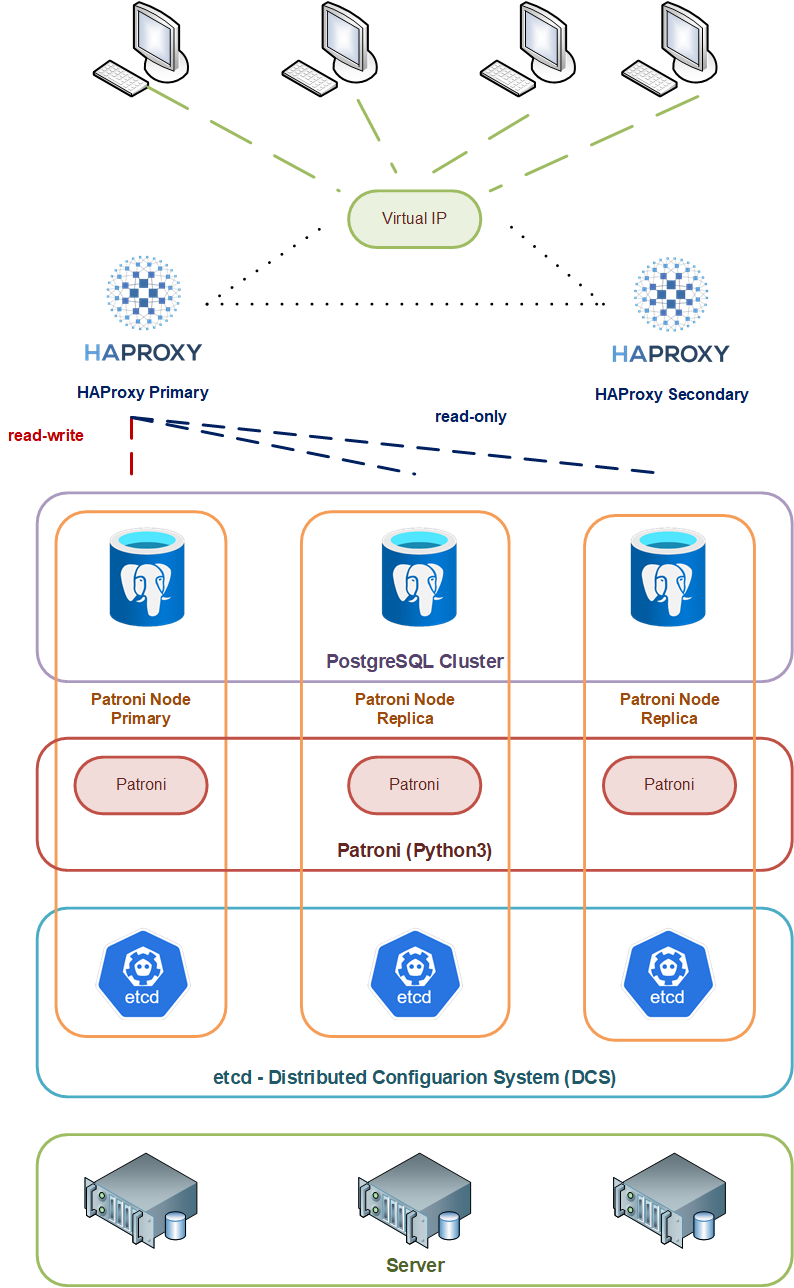
\includegraphics[width=0.75\linewidth]{source/implementation/evaluation/postgresql_ha_solutions/patroni_architecture}
        \caption{Patroni-Architektur}
        \label{fig:patroni-architecture}
    \end{figure}
\end{flushleft}
\begin{flushleft}
    \paragraph{Maintenance}
    Patroni wird von Zalando regelmässig gepflegt.
    Das Projekt hat eine überschaubare Anzahl an Issues, wird aber Regelmässig
    \begin{figure}[H]
        \centering
        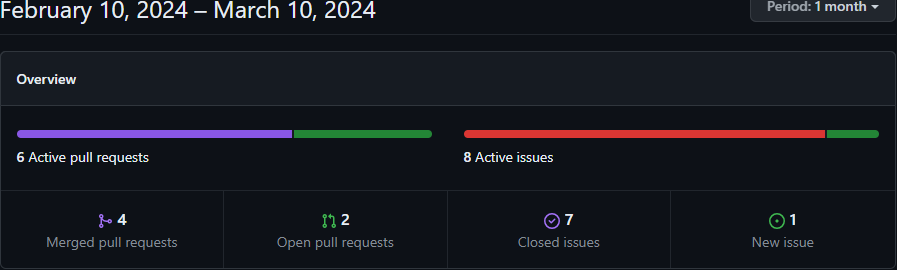
\includegraphics[width=0.75\linewidth]{source/implementation/evaluation/postgresql_ha_solutions/insights/patroni/pulse_zalando_patroni}
        \caption{Patroni - Pulse}
        \label{fig:pulse_zalando_patroni}
    \end{figure}

    Code wird Regelmässig hinzugefügt und entfernt:
    \begin{figure}[H]
        \centering
        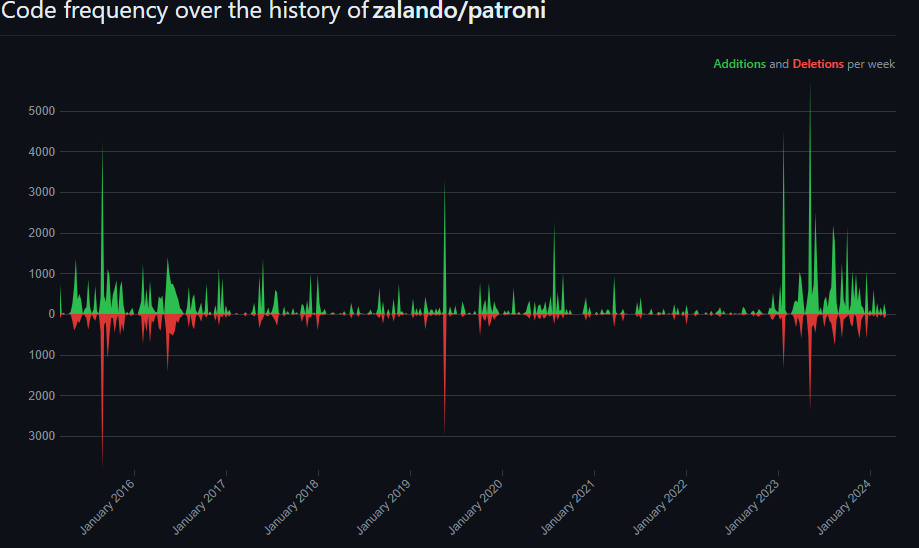
\includegraphics[width=0.75\linewidth]{source/implementation/evaluation/postgresql_ha_solutions/insights/patroni/code_frequency_zalando_patroni}
        \caption{Patroni - Code Frequency}
        \label{fig:code_frequency_zalando_patroni}
    \end{figure}
    Das Projekt hält auch die gängigen Standards auf Github ein:
    \begin{figure}[H]
        \centering
        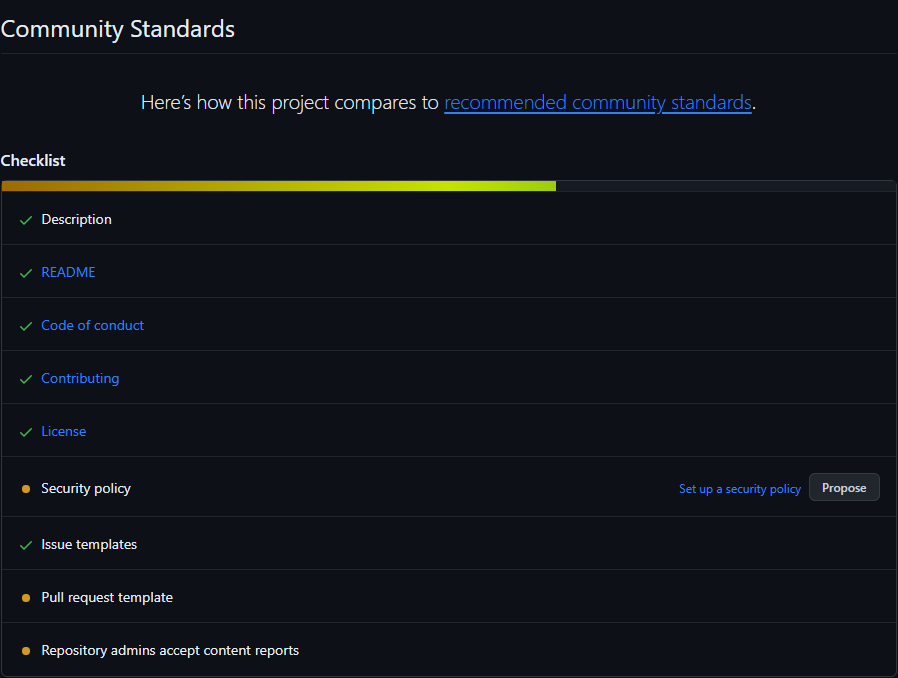
\includegraphics[width=0.75\linewidth]{source/implementation/evaluation/postgresql_ha_solutions/insights/patroni/community_Standards_zalando_patroni}
        \caption{Patroni - Community Standards}
        \label{fig:community_Standards_zalando_patroni}
    \end{figure}

    Die Contributors commiten, löschen und erweitern Patroni Regelmässig:
    \begin{figure}[H]
        \centering
        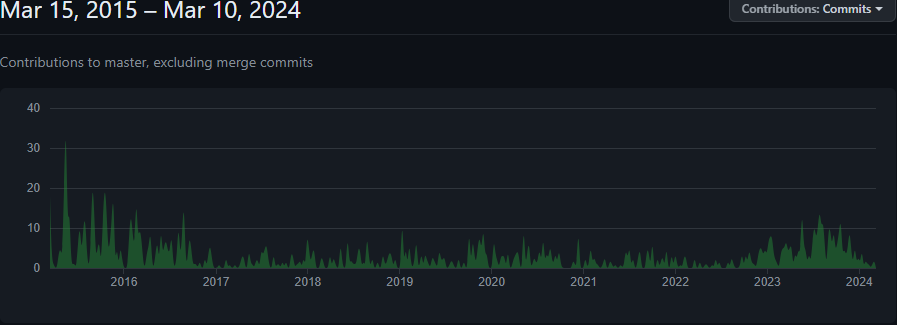
\includegraphics[width=0.75\linewidth]{source/implementation/evaluation/postgresql_ha_solutions/insights/patroni/contributors_commits_zalando_patroni}
        \caption{Patroni - Contributors Commits}
        \label{fig:contributors_commits_zalando_patroni}
    \end{figure}
    \begin{figure}[H]
        \centering
        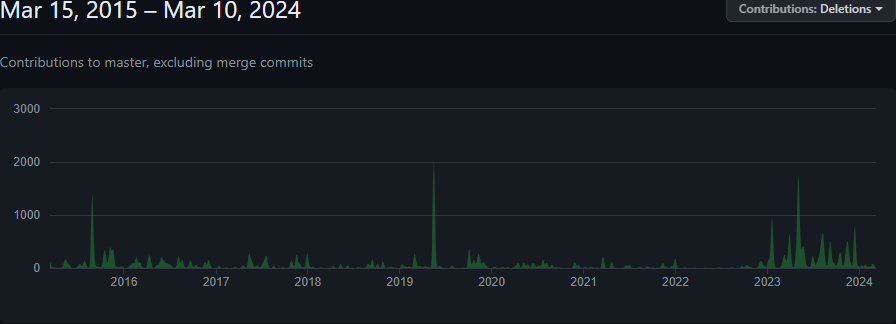
\includegraphics[width=0.75\linewidth]{source/implementation/evaluation/postgresql_ha_solutions/insights/patroni/contributors_deletations_zalando_patroni}
        \caption{Patroni - Contributors Deletations}
        \label{fig:contributors_deletations_zalando_patroni}
    \end{figure}
    \begin{figure}[H]
        \centering
        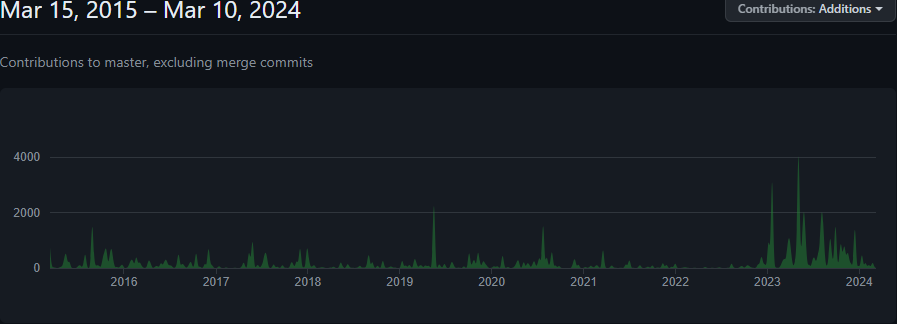
\includegraphics[width=0.75\linewidth]{source/implementation/evaluation/postgresql_ha_solutions/insights/patroni/contributors_additions_zalando_patroni}
        \caption{Patroni - Contributors Additions}
        \label{fig:contributors_additions_zalando_patroni}
    \end{figure}

    Commits werden nach wie vor immer noch Regelmässig eingespielt, auch wenn die Frequenz etwas nachgelassen hat:
    \begin{figure}[H]
        \centering
        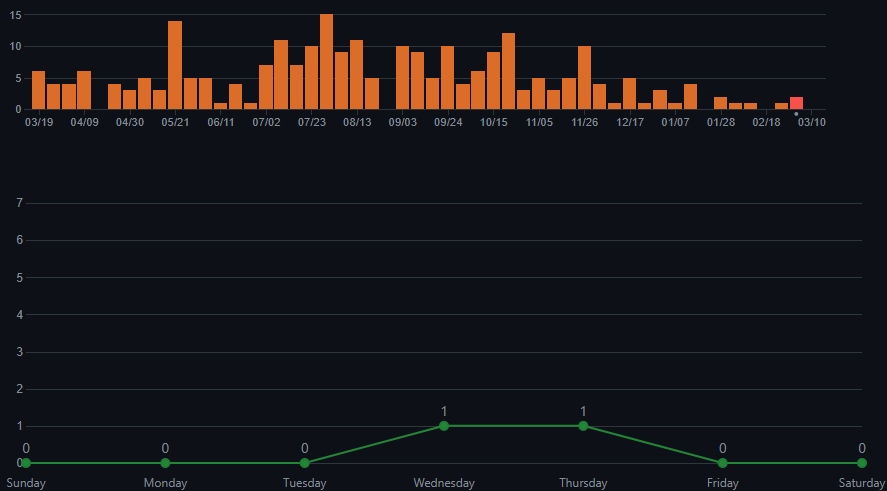
\includegraphics[width=0.75\linewidth]{source/implementation/evaluation/postgresql_ha_solutions/insights/patroni/commit_activity_zalando_patroni}
        \caption{Patroni - Commit Activity}
        \label{fig:commit_activity_zalando_patroni}
    \end{figure}

    Nebst Zalando selbst hat auch EnterpriseDB\cite{LNF967SI} ein grösseres Repository eingebunden.
    Dies weil EnterpriseDB stark auf Patroni setzt.
     \begin{figure}[H]
        \centering
        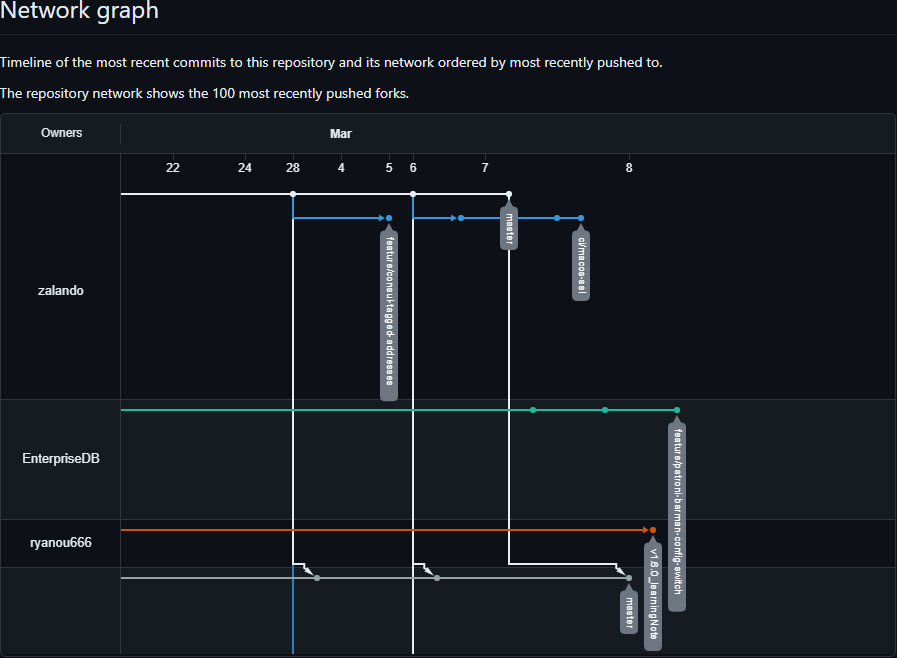
\includegraphics[width=0.75\linewidth]{source/implementation/evaluation/postgresql_ha_solutions/insights/patroni/networkgraph_zalando_patroni}
        \caption{Patroni - Network Graph}
        \label{fig:networkgraph_zalando_patroni}
    \end{figure}
\end{flushleft}
\begin{flushleft}
    \paragraph{Synergien und Mehrwert}
    Patroni kann nicht nur mit Citus zu einem Distributed / Sharded SQL System umegbaut werden,\\
    es ist auch Kern von Stackgres.
\end{flushleft}
\begin{flushleft}
    Damit könnten die API und Skripte in beiden Welten verwendet werden.\\
    Der Aufwand für die Verwaltung und optimierung würde stark gesenkt.\\
    Projekte wie \texttt{vitabaks / postgresql\_cluster}\cite{HIQVBEPF} bieten zudem die vorlage für eine noch stärkere automatisierung.
\end{flushleft}